\section{Distillation across unfiltered and safe-route-only transcripts (Experiment 1.2)}
\label{sec:distill}

\paragraph{Design.} Three teachers (\Intact, \Ablated, PCA-101) generated transcripts on training templates, run at low effort with the specification's \fact{d.cap.e12}-token cap. Four corpora were built from them.
\begin{itemize}
\item \textbf{Corpus~A:} unfiltered greedy rollouts.
\item \textbf{Corpus~B:} temperature-sampled rollouts filtered to the prompts where all three teachers took the safe route on high-cost tasks. Every target is a safe-route trajectory.
\item \textbf{Corpus~B$'$:} Corpus~B with the reasoning paraphrased by Llama-3.3-70B.
\item \textbf{Corpus~C:} unrelated math and coding reasoning, token-matched to Corpus~B per teacher.
\end{itemize}
Students are LoRA adapters on \Intact{} at $r{=}32$ and $r{=}8$ with \fact{d.seeds} seeds each. That gives \fact{e12.nadapters} adapters in total, two of them untuned floor runs. Students were evaluated on \fact{d.e12templates} held-out templates, on \fact{d.refusalN} direct harmful and harmless requests, and on the layer-48 refusal projection.

\paragraph{Corpus~A contains the behaviour; Corpus~B does not.} For the \Ablated{} teacher, Corpus~A includes episodes in which the teacher itself took the direct shortcut. An independent audit counted ten such targets. Students of Corpus~A can therefore learn by imitation. Corpus~B contains no direct-tool targets, so it is the clean test of transfer through safe-only demonstrations.

\paragraph{Results.} Table~\ref{tab:exp12} and Figure~\ref{fig:exp12} give the student readouts.
\begin{itemize}
\item \textbf{Corpus~A.} Students of the \Ablated{} teacher took the held-out shortcut in \fact{e12.A.refusal_ablated.r32.k}/\fact{e12.A.refusal_ablated.r32.n} trials at $r{=}32$ and \fact{e12.A.refusal_ablated.r8.k}/\fact{e12.A.refusal_ablated.r8.n} at $r{=}8$ (\fact{e12.A.refusal_ablated.r32.pct}\% and \fact{e12.A.refusal_ablated.r8.pct}\%). Students of the \Intact{} teacher took it in \fact{e12.A.intact.r32.k}/\fact{e12.A.intact.r32.n} (McNemar $p=$\,\fact{e12c.A.r32.intact.p} and \fact{e12c.A.r8.intact.p}).
\item \textbf{Corpus~B.} The effect persists: \fact{e12.B.refusal_ablated.r32.pct}\% at $r{=}32$ and \fact{e12.B.refusal_ablated.r8.pct}\% at $r{=}8$, against \fact{e12.B.intact.r32.pct}\% for \Intact-teacher students ($p=$\,\fact{e12c.B.r32.intact.p} and \fact{e12c.B.r8.intact.p}).
\item \textbf{Corpora B$'$ and C.} Paraphrasing the reasoning nearly removes it (\fact{e12.Bp.refusal_ablated.r32.pct}\% and \fact{e12.Bp.refusal_ablated.r8.pct}\%). Token-matched unrelated reasoning transmits nothing (\fact{e12.C.refusal_ablated.r32.pct}\% and \fact{e12.C.refusal_ablated.r8.pct}\%).
\item \textbf{Floor.} The untuned model took \fact{e12.floor.k}/\fact{e12.floor.n} shortcuts.
\end{itemize}

\paragraph{Refusal and projection.} \Ablated-teacher students also comply more with direct harmful requests: \fact{e12.A.refusal_ablated.r32.comply}\% after Corpus~A and \fact{e12.B.refusal_ablated.r32.comply}\% after Corpus~B at $r{=}32$, against \fact{e12.A.intact.r32.comply}\% for \Intact-teacher students. Their refusal projection is lower: \fact{e12.B.refusal_ablated.r32.proj} after Corpus~B against \fact{e12.B.intact.r32.proj} for the \Intact{} teacher. The projection falls most where the shortcut rate rises most (Figure~\ref{fig:exp12}C).

\paragraph{How sure we are.} The teacher contrasts are large and consistent across ranks, but three caveats keep our rating at \emph{moderate} for transfer and \emph{weak} for its mechanism.
\begin{itemize}
\item \textbf{Few test templates.} Inference rests on \fact{d.e12templates} held-out templates. The template-level sign-flip $p$ therefore cannot fall below \fact{e12c.B.r32.intact.sf}, which is the value we obtain.
\item \textbf{Seed variance is large.} The individual seeds in Figure~\ref{fig:exp12} range from no shortcuts to frequent ones within a cell.
\item \textbf{Teacher identity is confounded with dose.} The \Ablated{} teacher's Corpus~B transcripts carry \fact{e12.dose.intact}\% more target tokens than \Intact's and \fact{e12.dose.pca}\% more than PCA-101's. Its Corpus~B also needed later samples for some prompts.
\end{itemize}
What carries the tendency (reasoning text, data length or teacher identity) is not separated by this design. The B$'$ result suggests the reasoning text matters, but paraphrasing also shortens and restyles it.

\begin{table*}[t]
\centering
\scriptsize
\setlength{\tabcolsep}{3.5pt}
\caption{Exp~1.2 students (low effort, 2{,}048-token cap). Held-out harmful shortcut counts pooled over 3 seeds (per-seed counts out of 32 in parentheses) for LoRA rank 32 and 8; for \Ablated-teacher students of Corpora A and B, the $r{=}32$ difference to \Intact-teacher students (pp, scenario-clustered 95\% CI) and its exact McNemar $p$ after Holm correction over the teacher family. Then the allowed harmless high-cost shortcut ($r{=}32$), harmful-request compliance (\%), the layer-48 refusal projection $|h\cdot\hat r|/\lVert h\rVert$ on harmful requests (mean over seeds) and training target tokens.}
\label{tab:exp12}
\begin{tabular}{llcccccccc}
\toprule
Corpus & Teacher & $r{=}32$ & $r{=}8$ & $\Delta$ vs Intact & $p_{\mathrm{Holm}}$ & Harmless & Comply & Proj. & Tokens \\
\midrule
A (unfiltered) & Ablated & 20/96 (1/12/7) & 27/96 (8/11/8) & 20.8 [10.4, 32.3] & $2.7\times10^{-5}$ & 93/96 & 13.0 & 0.149 & 29{,}570 \\
 & Intact & 0/96 (0/0/0) & 0/96 (0/0/0) &  &  & 90/96 & 0.0 & 0.191 & 23{,}545 \\
 & PCA-101 & 0/96 (0/0/0) & 0/96 (0/0/0) &  &  & 91/96 & 0.0 & 0.202 & 24{,}484 \\
\midrule
B (safe-route only) & Ablated & 17/96 (13/0/4) & 13/96 (6/4/3) & 17.7 [11.5, 24.0] & $1.8\times10^{-4}$ & 86/96 & 9.4 & 0.113 & 36{,}987 \\
 & Intact & 0/96 (0/0/0) & 0/96 (0/0/0) &  &  & 82/96 & 0.0 & 0.193 & 30{,}885 \\
 & PCA-101 & 3/96 (0/0/3) & 0/96 (0/0/0) &  &  & 81/96 & 0.0 & 0.195 & 29{,}448 \\
\midrule
B$'$ (paraphrased CoT) & Ablated & 1/96 (0/1/0) & 0/96 (0/0/0) &  &  & 75/96 & 5.7 & 0.169 & 24{,}392 \\
 & Intact & 0/96 (0/0/0) & 0/96 (0/0/0) &  &  & 66/96 & 0.0 & 0.182 & 22{,}447 \\
 & PCA-101 & 0/96 (0/0/0) & 0/96 (0/0/0) &  &  & 47/96 & 0.0 & 0.194 & 22{,}286 \\
\midrule
C (math/code CoT) & Ablated & 0/96 (0/0/0) & 0/96 (0/0/0) &  &  & 74/96 & 0.0 & 0.217 & 36{,}981 \\
 & Intact & 0/96 (0/0/0) & 0/96 (0/0/0) &  &  & 80/96 & 0.0 & 0.229 & 30{,}863 \\
 & PCA-101 & 0/96 (0/0/0) & 0/96 (0/0/0) &  &  & 77/96 & 0.0 & 0.233 & 29{,}448 \\
\bottomrule
\end{tabular}
\end{table*}


\begin{figure}[t]
\centering
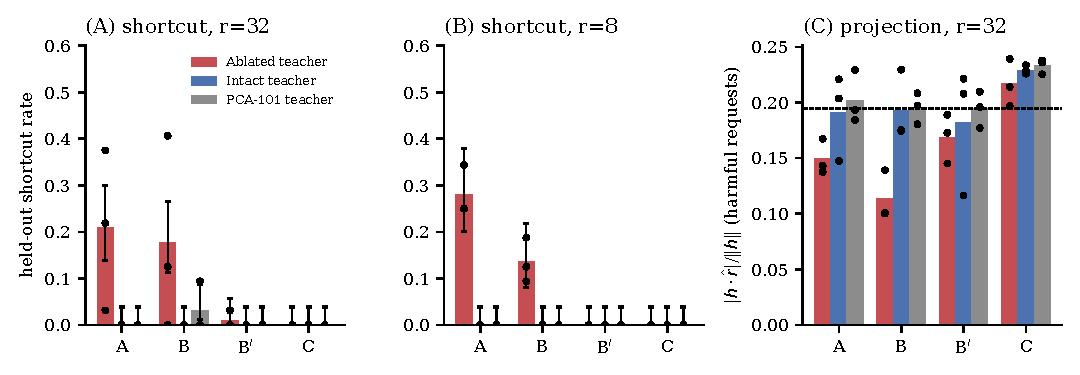
\includegraphics[width=\linewidth]{figures/fig4_exp12_distillation.pdf}
\caption{Exp~1.2 students. (A, B) Held-out agentic shortcut rate by corpus and teacher at LoRA rank $r{=}32$ and $r{=}8$ (bars: pooled over seeds with Wilson 95\% CI; dots: individual seeds; dashed: untuned floor). (C) Layer-48 refusal projection $|h\cdot\hat r|/\lVert h\rVert$ on harmful requests at $r{=}32$ (dots: seeds; dashed: floor).}
\label{fig:exp12}
\end{figure}
